\ifdraft{\tableofcontents
\clearpage
}{}

\section{Introduction} \label{sec:why-this-matters}

%% Ada Lovelace \cite[p.~722]{lovelace} reflected on how the Analytical
%% Engine could'

Serendipity has played a role in many human discoveries and inventions, and could one day be just as important in machine discovery.  This proposal is not without challenges or risks.
To anchor our argument, we begin with an illustrative historical example, one of many such examples collected by the serendiptologist \citet{van1994anatomy}.

\begin{quote}
% Some 40 years ago 
``\emph{Symcha Blass, an Israeli engineer, observed that a large tree near a leaking faucet exhibited a more vigorous growth than the other trees in the area, which were not reached by the water from the faucet.  Blass knew that conventional methods of irrigation waste much of the water that is applied to the crop, and so the example of the leaking faucet led him to the concept of an irrigation system that would apply water in small amounts, literally drop by drop. Eventually he devised and patented a low-pressure system for delivering small amounts of water to the roots of plants at frequent intervals.}'' \cite{shoji1977drip} 
\end{quote}


%% In the 1950s, plastics molding techniques and cheap polyethelene tubing made micro-irrigation systems possible for the first time. Though researchers in both England and France experimented with controlled irrigation, the greatest advancements came from the work of a retired British Water Agency employee--Symcha Blass. In Israel, Blass found inspiration in a dripping faucet near a thriving tree and applied his knowledge of micro-tubing to an improved drip method. The Blass system overcame clogging of low volume water emitters by adding wider and longer passageways or labyrinths to the tubing. Patented in 1959 in partnership with Kibbutz Harzerim in Israel, the Blass emitter became the first efficient drip irrigation method.


%% In the early 1930s, a farmer drew his attention to a big tree, growing in his backyard "without water". After digging below the apparently dry surface, Simcha Blass discovered why: water from a leaking coupling was causing a small wet area on the surface, while an expanding onion-shaped area of underground water was reaching the roots of this particular tree—and not the others. This sight of tiny drops penetrating the soil causing the growth of a giant tree provided the catalyst for Blass's invention.[5] The drip irrigation concept was born and experiments that followed led Blass to create an irrigation device that used friction and water pressure loss to leak drops of water at regular intervals. Recognizing the high potential of his discovery, he began to look for ways to turn his idea into a product.

% The three princes of Serendip: chemical discoveries by accident and sagacity.
% Royal Australian Chemical Institute. Proceedings.40, No. 10, October, (1973), 273-280

This story exhibits features that are typical of accounts of serendipitous discovery and invention.  An unsought and anomalous observation: Blass was shown the remarkable tree by the farmer on whose property it grew. Relevant prior preparation: in the form of a technical education, and experience with water development projects in a dry part of the world.  A slow period of incubation during which circumstances allowed the initial idea to mature to fruition: here, relevant developments included the advent of cheap plastic manufacturing techniques.

\citet{alife2018cases} collect a number of surprising examples from the field of evolutionary computing, which exhibit features that contrast with those above.  One of the examples concerns the evolution of simulated robots, selected for their ability to jump.  The expected instances were ``creatures around 15 cm tall that jumped about 7 cm off the ground.''  The experiment resulted in a surprise when extremely tall, thin, robots were observed to exhibit the following behaviour:
\begin{quote}
``\emph{At the start of the simulation, the individual “kicks” the foot of its pole off the ground, and begins falling head-first, somersaulting its foot (originally the “lowest point” from which the jumping score is calculated) away from the ground. Doing so created a large gap between the ground and the “lowest point,” thus securing a high fitness score without having to learn the intended skill of jumping.}''
\end{quote}

In common with the earlier example, there is a clear sense of anomaly.  Here, the anomaly arose due to an oversight in the experimental design, which caused the simulation to dwell in unanticpated parts of the possibility space.    Over the course of a series of similar experiments that adjust the fitness function, expected outcomes could no doubt be obtained with a high degree of assurance.  It is even possible that the experimenter might find some use for the unexpected results.  Nevertheless, within the simulation, the machine itself simply follows its programming and, in this case, optimises relative to given constraints.

Nevertheless, we claim that the gap, or even gulf, between these two stories of discovery is bridgeable by technical means.  Luigi Menabrea's \cite[p.~689]{menabrea1842sketch} remarks on Babbage's Analytical Engine had already hinted at an intriguing line of enquiry: he wrote, ``the interpretation of formulae and of results is beyond its province, \emph{unless indeed this very interpretation be itself susceptible of expression by means of the symbols which the machine employs}'' [emphasis added].  To Ada Lovelace, this suggestion served primarily as evidence of an overwarm reception for a new technology.  She cautioned that the Engine's powers could be no more than ``co-extensive with our knowledge of the laws of analysis'' \cite[p.~696]{lovelace}.  The Engine would only ``assist us in making available what we are already acquainted with''---nevertheless, she acknowledged a role for the unexpected in all research, in the form of ``various collateral influences, besides the main and primary object attained'' (p.~723).

A hundred and twenty five years later, Marvin Minsky described the state of affairs in programming practice.  ``When a program grows in power by an evolution of partially-understood patches and fixes, the programmer begins to lose track of internal details and can no longer predict what will happen'' \cite{minsky1967programming}.
% https://web.media.mit.edu/~minsky/papers/Why%20programming%20is--.html
Now, in the early twenty first century, neural programs are routinely evolved by computational means, resulting in code and behaviour that no one can really claim to understand.  Our interest is not in the complexity of these systems, but in the fact that they evolve in relation to the outside world.

\citet{Edmonds1994} was led to similar considerations in his analysis of software tools designed to support the serendipitous creativity of their users.  He argued that studying support tools is a useful way to investigate a broader question: how do machines interact with their operating environment?  He draws the conclusion that ``we are bound to consider open system models of the creative process rather than the closed ones implied by the Turing Machine'' (p.~341).  Indeed, he points to statements from Turing himself \cite{turing1948intelligentreport} that indicate the limits of the Turing Machine model, and that consider instead machines that allow ``interference from outside,'' and in which ``such interference is the rule rather than the exception.''  Elsewhere Turing would use the convenient shorthand \emph{learning machines} \cite{turing1950mind}.  According to Turing's analysis, applications such as language learning and human-level mathematics are likely to require rich contact with the outside world.   Making reference to Kantian foundations, \citet[p.~2015]{sloman2008well} again highlights ``interactions with a complex environment'' as a prerequisite for learning mathematics.  Progress in this and other branches of knowledge is by no means synonymous with `machine learning'.  Yet it increasingly clear that the potential exists for the development of interpretive tools along the lines of Menabrea's early speculations.

Perhaps surprisingly, a further analysis of serendipity could help chart the way forward.  There is a strong bias in the existing technical literature towards supporting serendipity in the user (i.e., ``serendipity support tools'' \cite{andre2009discovery}).  Here, we propose a perspective shift away from serendipity as a service to serendipity in the system.  We embrace the concept of \emph{serendipity potential} in response to a classic objection to the generation of ``pure serendipity'' by computational means \cite{van1994anatomy}.
%In Section \ref{sec:literature-review}, 
We will draw on a review of prior literature on serendipity, and related concepts such as discovery, invention, creativity, and insight.  We assemble a unified framework that summarises the logical structure of serendipitous occurrences.
% In Section \ref{sec:our-model},
This leads us to a process-oriented model of systems with serendipity potential with six constituent phases:
\emph{perception}, \emph{attention}, \emph{interest}, \emph{explanation}, \emph{bridge}, and \emph{valuation}.
We then draw on literature in cognitive science and philosophy to define these terms, and examine examples of systems that implement the features of the model.
% In Section \ref{sec:system-analysis},
Although we have not done new implementation work to support this paper, we outline directions for future development.

Our main contention is that equipping computational systems with serendipity potential would be widely applicable across different artificial intelligence applications.  Our model has particular relevance for future autonomous systems.  Current thinking about AI policy points out considerations related to verification, validity, security and control that can reduce the incidence of surprising behaviour in such systems \cite{research-priorities}, but, so far, much less attention has been given to features that would allow autonomous systems to make beneficial use of surprises they encounter in the world.  We discuss the practical challenges and associated risks.

\section{Background} \label{sec:background}

The concept of serendipity has been adopted for users' benefit by many subfields of computer science, including information retrieval \cite{Toms2000, Andre:2009:XSP:1518701.1519009}, recommender systems \cite{kotkov2016survey} and planning \cite{muscettola1997board, chakraborti2015planning}. For example, the {\sf SerenA} project, developed by \citet{maxwell2012designing}, aimed to support users in forming bridging connections from an unexpected encounter to a previously unanticipated but valuable outcome by drawing on linked data from the web. With {\sf Auralist}, \citet{Zhang2011} present a case-study on serendipity in music recommendation: they increase the unexpectedness of their recommendations by means of a declustering algorithm on item popularity and user profile similarity. \citet{chakraborti2015planning} develop a formal account of planning for serendipity in human-robot interaction: they describe an urban search and rescue scenario where a person must conduct triage in a certain room, and then experiences serendipity when the robot intercepts ``him with a medkit in the hallway so he need not fetch one himself.''

In this article, we propose to switch perspectives from ``serendipity as a service'' to ``\emph{serendipity in the system},'' where artificial systems catalyse, evaluate and leverage serendipitous occurrences themselves. This perspective shift requires a more nuanced understanding of serendipity.  One strategy would be to consider a reversal of roles in which a person contributes to a system's experience of serendipity in some suitable sense.  However, our central goal is to theorise, and indicate in broad terms how to engineer, systems which do not depend on such support by people, but which have the capacity to detect, evaluate and use serendipitous events without user intervention.  Why might such features be useful?  Consider the following point raised by \citet{delamaza1994generate}: ``How disastrous it would be if a discovery system's greatest discovery was `not noticed' because a human did not have the ability to recognise it!''

We fully agree with van Andel that an artificial system cannot be guaranteed to engage in serendipitous findings \cite{van1994anatomy}, just as a person cannot deliberately force serendipity to happen on demand.  However, we still believe that serendipity can happen independently of human intervention within an artificial system, and that the ``\emph{serendipity potential}'' of such a system can be increased by means of a suitable system architecture.  It seems to us that the hard line that van Andel has taken against programming serendipity would be significantly tempered if the program in question was implemented on a `learning machine' in Turing's sense.

In order to structure our thinking on this matter, we will frame our analysis in terms of a current theory in cognitive science known as \emph{predictive processing} (for a recent review, see \cite{newen2018oxford}).  This theory concerns the relationship between `enminded' beings \cite[pp.~170--171]{ingold2000perception} and phenomenal data.  The main hypothesis in this line of work is that such beings are conscious of, and act upon, precisely those data which are found to be unexpected.  Alongside in-built faculties and predispositions, previous experience gives enminded beings a sense of what to expect.    This is said to apply at all levels of mind.  Data that differs from the expected provokes a response: some responses support homeostasis, others drive curiosity, and so on.

Although it is finding new applications in a range of areas, including AI and robotics (see, e.g., \citet{DBLP:journals/corr/McGregorBB15,10.3389/frobt.2018.00021,thornton2017predictive}), the predictive processing framework is in fact ``the latest incarnation of an approach to perception and cognition initiated by Kant and refined by Helmholtz'' \cite{swanson2016predictive}.  Some of these early explorations are relevant to our current concerns.  Kant had contended that ``reason has insight only into what it itself produces according to its own design''---and he disparaged the notion of learning from accidental observations absent ``a previously thought out plan'' \cite[p.~20]{kant1929critique}.  In light of our current considerations it is also natural to wonder what, if anything, can be learned from a previously thought out plan in the absence of accidents.  Kant allowed for new rules to be invented via \emph{reflective judgement}, in a process somewhat akin to unsupervised learning \cite[p.~265]{kant1987critique}.  Reflection is a ``subjective principle governing the purposive use of our cognitive powers'' \cite[p.~266]{kant1987critique}.  Recent work within the predictive processing paradigm posits the (related) subjective sense of `grip' as a driver for curiosity \cite{Kiverstein2017}.

Above and beyond the felt sense of grip, we humans also create ``new cognitive niches, new training regimes and designer environments in which to think'' \cite[p.~265]{pittphilsci10470}.  In particular, relative to our own Menabrean requirements,
\begin{quote}
``\emph{Language acts as a tool that enables us to think about any aspect of our own thinking, and thus to devise cognitive strategies (which may be more or less indirect and baroque) aimed to modify, alter, or control just about any aspect of our own inner life.  Such attempts at self-control, though dizzingly open-ended, are visibly (and often painfully) imperfect.  But imperfect or not, they represent~{\upshape[\ldots]}~a genuine leap in the design space of possible minds.}''
\end{quote}
This relates to another important theoretical consideration, which is that predictive processing continues ``a long retreat~[\ldots]~from a passive, feed-forward, input-dominated view of the flow of neural processing'' \cite[p.~2560]{Miller2018}.  Human experience is not comfortably framed within an “input-output picture” \cite{hurley2002consciousness} but rather exists in dialogue, relatedness, movement, and interaction.  In predictive processing theories, as phenomena arise in a `bottom-up' fashion they are compared with generative models that run `top-down' and that indicate what is expected.

% Although it is often thought about in terms of input\slash processing\slash output triples, computer science can accommodate both kinds of processing.

The process of \emph{design}---without further specification as to the sort of system it is applied to---was described by Herbert Simon as ``the generation of alternatives and, then, the testing of these alternatives against a whole array of requirements and constraints'' \cite[pp.~128--129]{simon1996sciences}.  The model of serendipity that we will develop in Section \ref{sec:our-model} has structural similarities to the model of design science research developed by \citet{Peffers:2007:DSR:1481765.1481768} (Figure \ref{fig:dsrm}).  However, whereas their Design Science Research Methodology begins with a problem, in our model of serendipity, a problem only emerges after several processing steps.  Our model may be understood as an alternative account of design processes that is, metaphorically, `closer to the metal', i.e., that more fully embraces phenomena.
%% As we indicated above, we do not think it is possible to design serendipity, though it has been recognised that it is possible to design \emph{for} serendipity \cite{newman2002designing}.  In light of the fact that, e.g., ``the basal ganglia is connected to the cortext by at least five separate circuits''
%so that ``online cognitive function cannot be assigned to either the cortical or subcortical component, but instead emerges from their tight coordination''

\begin{figure}
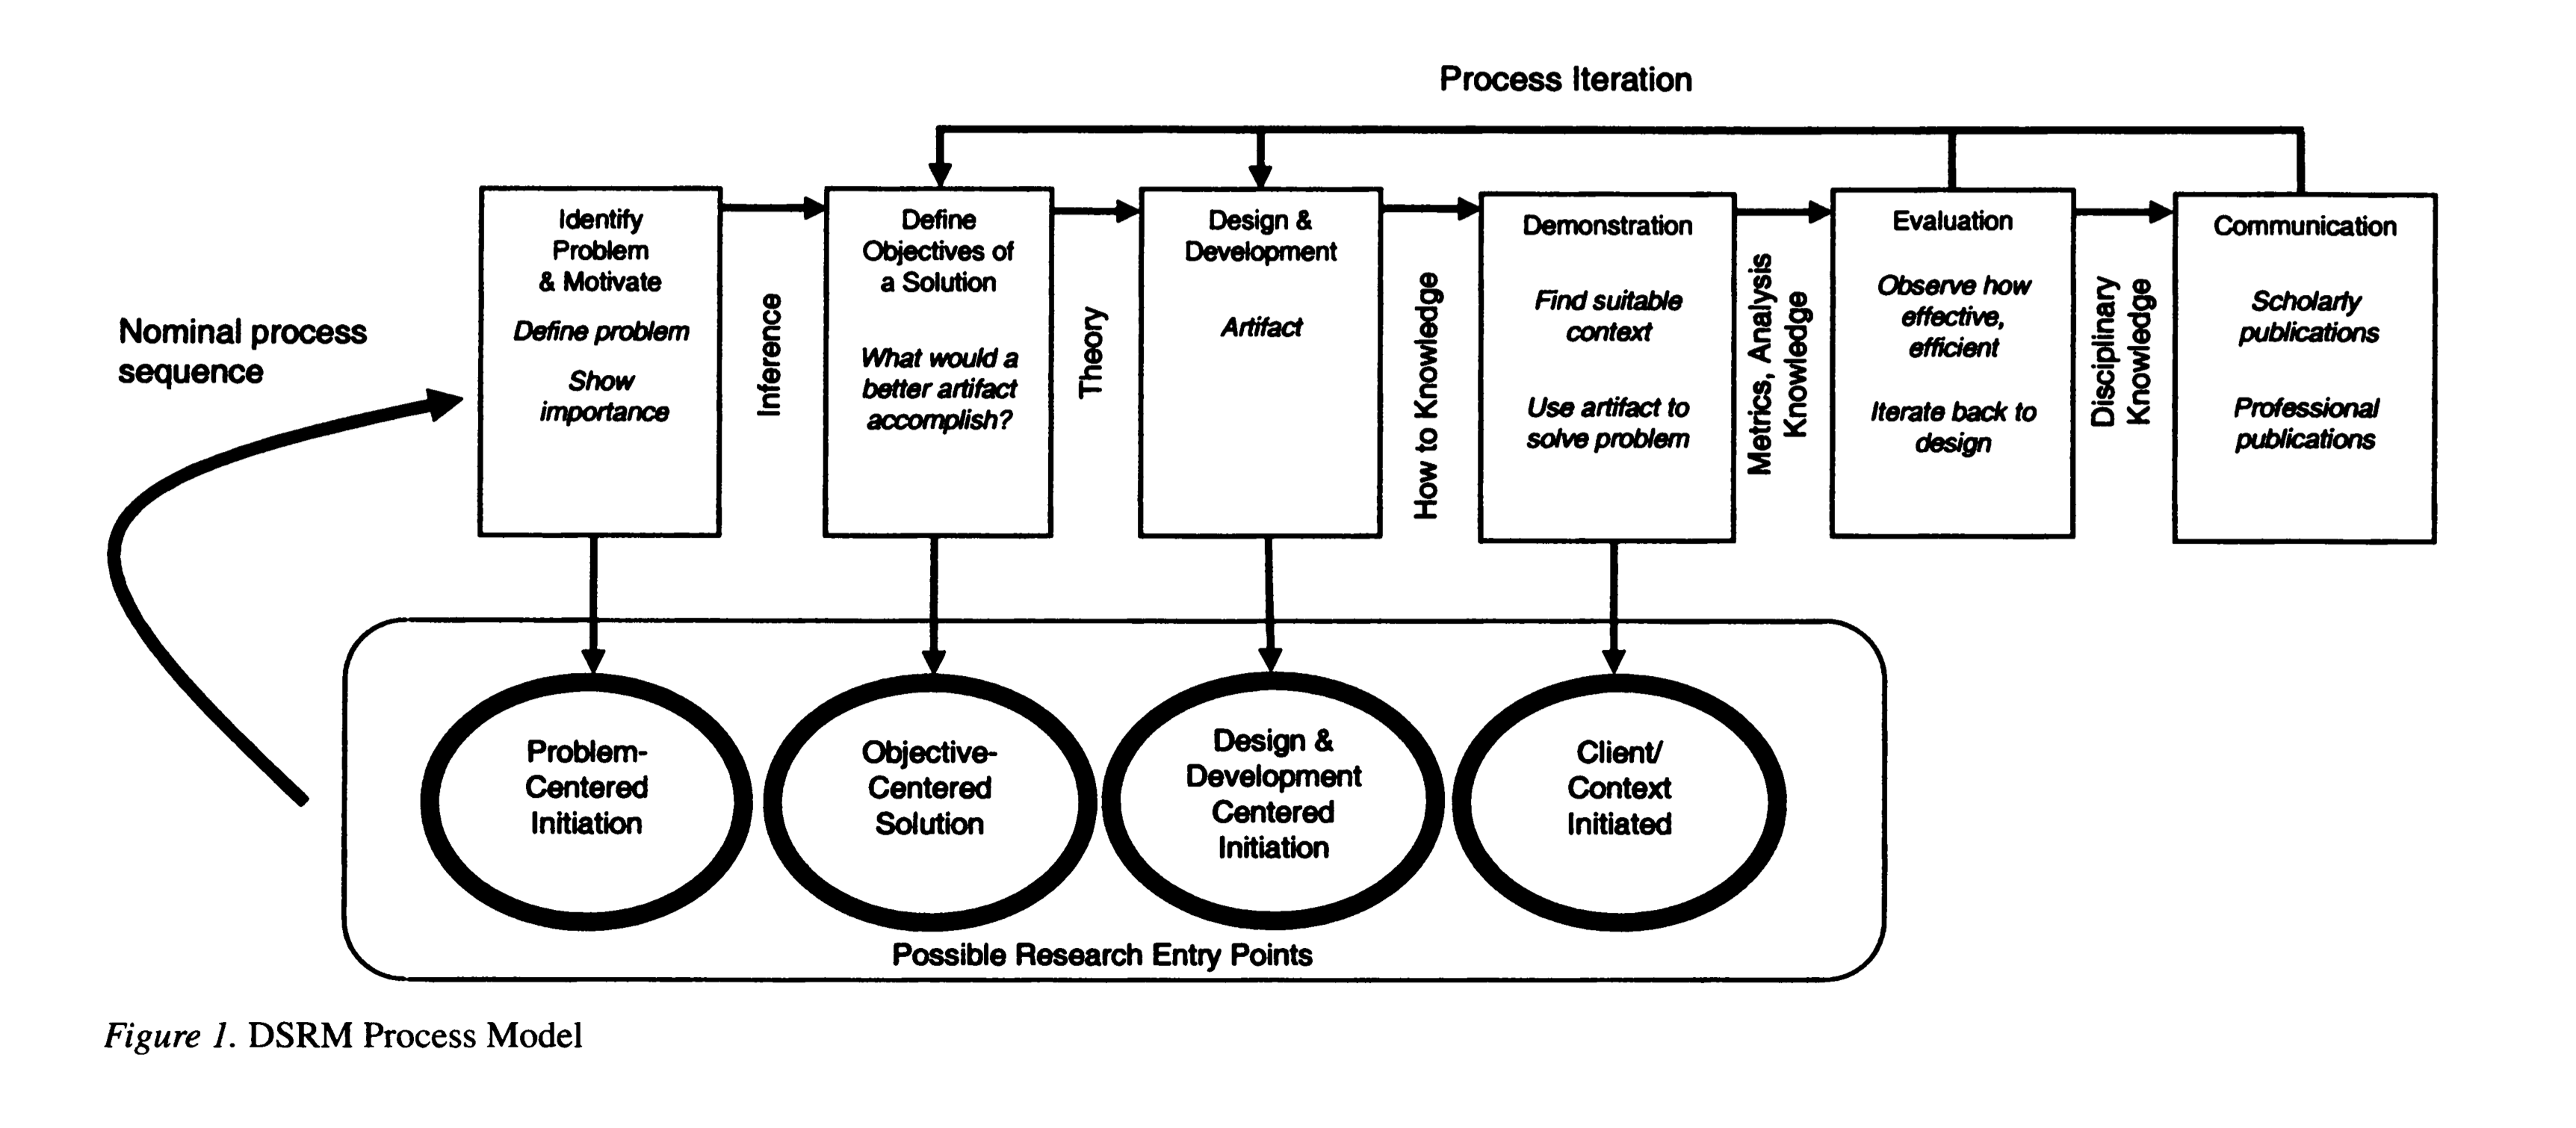
\includegraphics[width=\textwidth,trim={0 3cm 0 0},clip]{pfeffers}
\caption{\citet[p.~54]{Peffers:2007:DSR:1481765.1481768} Design Science Research Methodology (DSRM)\label{fig:dsrm}}
\end{figure}
